\documentclass{standalone}
\usepackage{tikz}
\usetikzlibrary{arrows.meta}
\tikzset{label/.style = {inner sep=1pt, fill=white}}
%\tikzset{nd/.style={circle, inner sep=0pt}}
\tikzset{nd/.style={inner sep=1pt}}
\tikzset{>=Latex}
\tikzset{arc/.style = {->, semithick, >=Latex}}
\begin{document}
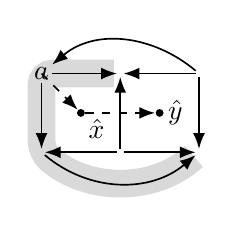
\begin{tikzpicture}

\draw [rounded corners, color = gray!30, line width = 10pt] (0,2) -- (1,2) -- (0,2) -- (0,1) to[in = 220, out = -40] (2,1) to[out = 220, in = -40] (0,1) -- cycle;

    \node[nd] (4) at (0,1) {};
    \node[nd] (5) at (1,1) {};
    \node[nd] (6) at (2,1) {};
    \node[nd] (7) at (0,2) {$a$};
    \node[nd] (8) at (1,2) {};
    \node[nd] (9) at (2,2) {};
    
    %\draw[arc] (4) to (1);
    %\draw[arc] (3) to[in = -40, out = 220] (1);
    \draw[arc] (9) to (8);
    \draw[arc] (5) to (8);
    \draw[arc] (5) to (4);
    
    \draw[arc] (7) to (4);
    %\draw[arc] (7) to[in = 130, out = -130] (1);
    \draw[arc] (7) to (8);
    \draw[arc] (9) to[out = 140, in = 40] (7);
    %\draw[arc] (1) to (2);
    \draw[arc] (9) to (6);
    \draw[arc] (5) to (6);
    \draw[arc] (4) to[in = 220, out = -40] (6);

    \node[nd, circle, inner sep= 1pt, fill] (x) at (0.5,1.5) {};
    \node at (0.7,1.3) {$\hat x$};

    \node[nd, circle, inner sep= 1pt, fill] (y) at (1.5,1.5) {};
    \node at (1.7,1.5) {$\hat y$};

    \draw[arc,dashed] (0,2) to (x);
    \draw[arc,dashed] (x) to (y);
    
 \end{tikzpicture}
\end{document}